\documentclass{article}
\usepackage{graphicx} % Required for inserting images
\usepackage{enumitem}
\usepackage{xcolor}
\usepackage{listings}

\setlength{\oddsidemargin}{-0.25in}
\setlength{\topmargin}{-0.5in}
\setlength{\headheight}{0cm}
\setlength{\headsep}{0cm}
\setlength{\textheight}{10in}
\setlength{\textwidth}{7in}
\setlength{\topskip}{0cm}

\begin{document}

\noindent\textbf{ComS 472 - PS3 \quad Due: Sept 29, 2024 \quad Name: Aren Ashlock}

\begin{enumerate}

% ------------------------------------- 1 DONE -------------------------------------

\item \textbf{(10 pts)} (Exercise 4.1) Give the name of the algorithm that results from each of the following special cases:

    \begin{enumerate}[label=($\alph*$)]
    
    % --------------------------------- 1a NOT DONE ---------------------------------
    
    \item \textbf{(2 pts)} Local beam search with $k = 1$.

    \color{blue}
        \textbf{Hill Climbing}, since the singular best next state is the one that is chosen to be kept.
    \color{black}

    % -------------------------------------------------------------------------------

    % ----------------------------------- 1b DONE -----------------------------------

    \item \textbf{(2 pts)} Local beam search with one initial state and no limit on the number of states retained.

    \color{blue}
        \textbf{Breadth-First Search}, because all possible actions are explored since all successor states are kept.
    \color{black}

    % -------------------------------------------------------------------------------

    % ----------------------------------- 1c DONE -----------------------------------

    \item \textbf{(2 pts)} Simulated annealing with $T = 0$ at all times (and omitting the termination test).

    \color{blue}
       \textbf{Hill Climbing}, because worse states will never end up being chosen, so it can only go up
    \color{black}

    % -------------------------------------------------------------------------------

    % ----------------------------------- 1d DONE -----------------------------------

    \item \textbf{(2 pts)} Simulated annealing with $T = \infty$ at all times.

    \color{blue}
        \textbf{Depth-First Search}, since a random successor state is chosen at each step whether better ($\Delta E > 0$, which better actions are always chosen) or worse ($e^{\Delta E / \infty} = 1$, so even a worse action is always chosen). It'll end up exploring as deep as it can get.
    \color{black}

    % -------------------------------------------------------------------------------

    % ----------------------------------- 1e DONE -----------------------------------
    \item \textbf{(2 pts)} Genetic algorithm with population size $N = 1$.

    \color{blue}
        \textbf{Depth-First Search}, this is because there is only 1 state being chosen for both parents, so the only change may come from a random mutation. The situation for this problem is similar to the previous one given that it'll explore a singular child and go as deep as it can.
    \color{black}

    % -------------------------------------------------------------------------------
    
    \end{enumerate}

% ----------------------------------------------------------------------------------

% ----------------------------------- 2 NOT DONE -----------------------------------

\item \textbf{(15 pts)} (Exercise 4.8) This exercise explores subset–superset relations between belief states in sensorless or partially observable environments.

\begin{enumerate}[label=($\alph*$)]
    
    % ----------------------------------- 2a DONE -----------------------------------
    
    \item \textbf{(2 pts)} Argue that if an action sequence is a solution for a belief state $b$, it is also a solution for any subset of $b$.

    \color{blue}
        Every state in a subset of a belief state is contained in the superset's belief state. For example, in the non-erratic vacuum world, the initial belief state contains $\{1, 2, 3, 4, 5, 6, 7, 8\}$. Both subsets $\{1, 3, 5, 7\}$ and $\{2, 4, 6, 8\}$ only contain states that are also in the initial belief state. Since there is a solution to that initial belief state, nothing changes by narrowing the belief state. Since the solution works from any of the initial 8 states, either subset containing only states from that initial group will ultimately work.
    \color{black}

    % -------------------------------------------------------------------------------

    % ----------------------------------- 2b DONE -----------------------------------

    \item \textbf{(5 pts)} Can anything be said about supersets of $b$ in (a)?

    \color{blue}
        We know that the supersets of $b$ have AT LEAST 1 solution, therefore it is solvable. Since it is a superset, that means there exists at least 1 action sequence to reach $b$, which we already know has a solution to it. That being said, s superset will contain elements not found in $b$. Meaning, it's not guaranteed that ALL subsets of the superset of $b$ will be a solution. 
    \color{black}

    % -------------------------------------------------------------------------------

    % ----------------------------------- 2c DONE -----------------------------------
    
    \item \textbf{(4 pts)} Explain in detail how to modify graph search for sensorless problems to take advantage of your answers in (a) and (b).

    \color{blue}
        The first thing I'd modify is if I knew there was a solution for a belief state, I would prune the other subsets that don't correspond to the action sequence. Since we only care about finding a solution, the other subsets are unnecessary whether they also provide a solution or not. By keeping them, the search may come to a dead end. Then, since we are only worried about reaching that known belief state, I'd focus on expanding the supersets of the solved belief state to find which actions in any state of the superset results in the solved belief state. You can repeat these 2 things until your belief state becomes the initial belief state, which now has a solution.
    \color{black}

    % -------------------------------------------------------------------------------

    % ----------------------------------- 2d DONE -----------------------------------
    
    \item \textbf{(4 pts)} Explain in detail how to modify and–or search for partially observable problems, beyond the modifications you describe in (c).

    \color{blue}
        Since the environment is partially observable, we can gain smaller belief states since it's possible to perceive some aspect(s) of the environment. Therefore, the action sequence will result in further subsets, which we can prune those since we know that a solution exists for the initial belief state, there exists some solution for any of the produced subsets. So we only need to focus on singular subsets.
    \color{black}

    % -------------------------------------------------------------------------------

    \end{enumerate}

% ----------------------------------------------------------------------------------

% ------------------------------------- 3 DONE -------------------------------------

\item \textbf{(7 pts)} (Exercise 4.10) Consider the sensorless version of the erratic vacuum world. Draw the belief-state space reachable from the initial belief state \{1, 2, 3, 4, 5, 6, 7, 8\}, and explain why the problem is unsolvable.

\begin{center}
    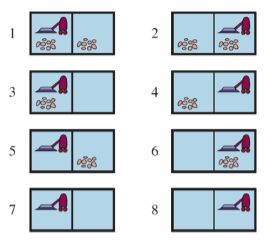
\includegraphics[scale=0.75]{472-PS3-Q3.png}
\end{center}

\color{blue}
    Below is the belief-state space, which contain all possible belief states. Since there are no states possible that contain only state 7, state 8, or just states 7 and 8, this problem is unsolvable. This is because the erratic vacuum world introduces non-determinism and that is unsolvable in a partial-perception environment where the vacuum doesn't know the amount of dirt in each square.
\color{black}

\begin{center}
    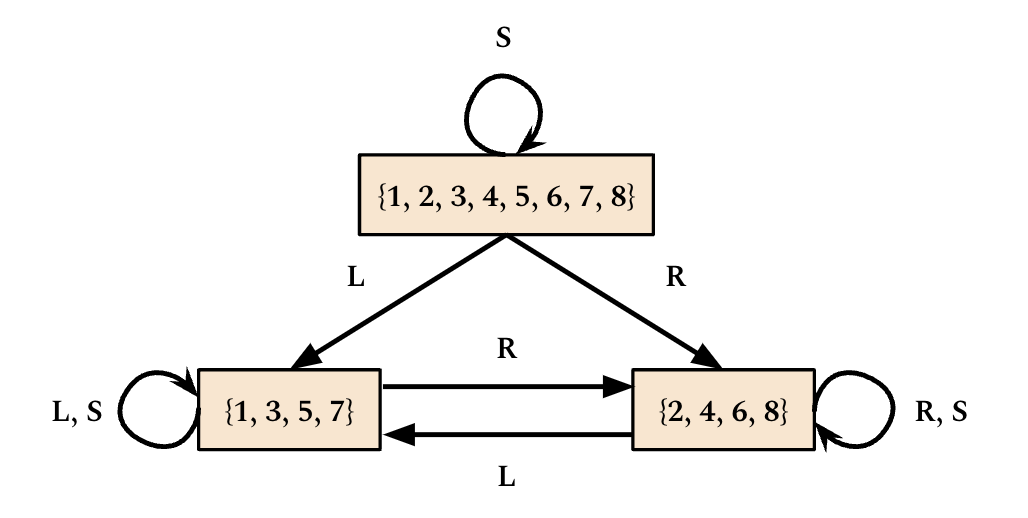
\includegraphics[scale=0.75]{472-PS3-Q3-answer.png}
\end{center}

% ----------------------------------------------------------------------------------

% ------------------------------------- 4 DONE -------------------------------------

\item \textbf{(8 pts)} Shown below is the AND-OR graph representation of the state space of a search problem, which has five states $S_0, S_1, S_2, S_3, S_g$ and five actions $a_1, a_2, a_3, a_4, a_5$. Here, $S_0$ is the initial state and $S_g$ is the goal state. (The structure is a graph because a state can be reached from multiple other states.) It is known that some of the actions may be erratic in non-deterministically generating an outcome state.

\begin{center}
    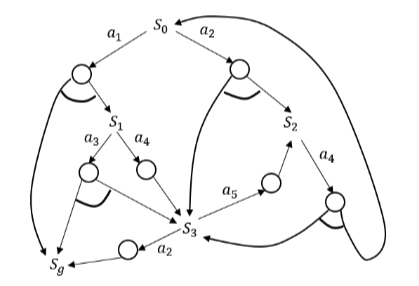
\includegraphics[scale=0.75]{472-PS3-Q4.png}
\end{center}

Give a solution to this problem. You may draw a closed contour around the subgraph that represents the solution. Or you may write down a conditional plan that uses atomic statements which are actions, and \textbf{if-then} or \textbf{if-then-else} statements whose conditions are states.

\color{blue}
\begin{lstlisting}
take a_1
if(state = S_g)
    then done
    else
        take a_4
        take a_2
        done
\end{lstlisting}
\color{black}

% ----------------------------------------------------------------------------------

\end{enumerate}
\end{document}